
 \documentclass[12pt]{article}
\usepackage{graphicx}
\usepackage{booktabs}
 \usepackage{makecell}
 \usepackage{float}
 \newcommand{\diff}{\,\mathrm{d}}
\usepackage[margin=1in]{geometry}
\usepackage{fancyhdr}
\pagestyle{fancy}
\usepackage{extarrows}
\usepackage{breqn}

\newcommand{\N}{\mathbb{N}}
\newcommand{\Z}{\mathbb{Z}}
\newcommand{\trans}{^{\mathrm T}}
\usepackage{amssymb}
\usepackage[table]{xcolor}
\usepackage{bm}
\usepackage{array}
\usepackage{mathtools}
\usepackage[english]{babel}
\usepackage{natbib}
\usepackage{url}
\usepackage[utf8x]{inputenc}
\usepackage{amsmath}
\usepackage{graphicx}
\graphicspath{{images/}}
\usepackage{parskip}
\usepackage{fancyhdr}
\usepackage{vmargin}
\usepackage[font={bf, footnotesize}, textfont=md]{caption}
\usepackage{amsmath,amsthm,amssymb}


\newenvironment{theorem}[2][Theorem]{\begin{trivlist}
\item[\hskip \labelsep {\bfseries #1}\hskip \labelsep {\bfseries #2.}]}{\end{trivlist}}
\newenvironment{lemma}[2][Lemma]{\begin{trivlist}
\item[\hskip \labelsep {\bfseries #1}\hskip \labelsep {\bfseries #2.}]}{\end{trivlist}}
\newenvironment{exercise}[2][Exercise]{\begin{trivlist}
\item[\hskip \labelsep {\bfseries #1}\hskip \labelsep {\bfseries #2.}]}{\end{trivlist}}
\newenvironment{reflection}[2][Reflection]{\begin{trivlist}
\item[\hskip \labelsep {\bfseries #1}\hskip \labelsep {\bfseries #2.}]}{\end{trivlist}}
\newenvironment{proposition}[2][Proposition]{\begin{trivlist}
\item[\hskip \labelsep {\bfseries #1}\hskip \labelsep {\bfseries #2.}]}{\end{trivlist}}
\newenvironment{corollary}[2][Corollary]{\begin{trivlist}
\item[\hskip \labelsep {\bfseries #1}\hskip \labelsep {\bfseries #2.}]}{\end{trivlist}}
\DeclareMathOperator{\tr}{tr}
\DeclareMathOperator{\rank}{rank}
\DeclareMathOperator{\Span}{span}
\DeclareMathOperator{\row}{row}
\DeclareMathOperator{\col}{col}
\DeclareMathOperator{\range}{range}
\DeclarePairedDelimiterX{\inp}[2]{\langle}{\rangle}{#1, #2}
\DeclareMathOperator{\Proj}{Proj}
\DeclareMathOperator{\trace}{trace}
\newcommand{\Her}{^{\mathrm H}}
\DeclareMathOperator{\diag}{diag}
\makeatletter 
    \newcommand\fcaption{\def\@captype{table}\caption}
\makeatother
\setmarginsrb{3 cm}{2.5 cm}{3 cm}{2.5 cm}{1 cm}{1.5 cm}{1 cm}{1.5 cm}

\title{Lab Report for PHY 1002 Guideline}                             % Title
\author{Name of Author}                               % Author
\date{\today}                                           % Date

\makeatletter
\let\thetitle\@title
\let\theauthor\@author
\let\thedate\@date
\makeatother

\pagestyle{fancy}
\fancyhf{}
\rhead{\theauthor}
\lhead{\thetitle}
\cfoot{\thepage}

\begin{document}

%%%%%%%%%%%%%%%%%%%%%%%%%%%%%%%%%%%%%%%%%%%%%%%%%%%%%%%%%%%%%%%%%%%%%%%%%%%%%%%%%%%%%%%%%

\begin{titlepage}
    \centering
    \vspace*{0.5 cm}
    
\includegraphics[scale = 0.75,width=6cm]{CUHK}\\[1.0 cm]   % University Logo
    \textsc{\large The Chinese University of Hong Kong, Shenzhen}\\[2.0 cm]   % University Name
    \textsc{\Large PHY 1002}\\[0.5 cm]               % Course Code
    \textsc{\large Physics Laboratory}\\[0.5 cm]               % Course Name
    \rule{\linewidth}{0.2 mm} \\[0.4 cm]
    { \huge \bfseries \thetitle}\\
    \rule{\linewidth}{0.2 mm} \\[1.5 cm]
    
    \begin{minipage}{0.4\textwidth}
        \begin{flushleft} \large
            \emph{Author:}\\
            \theauthor
            \end{flushleft}
            \end{minipage}~
            \begin{minipage}{0.4\textwidth}
            \begin{flushright} \large
            \emph{Student Number:} \\
            116010000                                   % Your Student Number
        \end{flushright}
    \end{minipage}\\[2 cm]
    
    {\large \thedate}\\[2 cm]
 
    \vfill
    
\end{titlepage}

%%%%%%%%%%%%%%%%%%%%%%%%%%%%%%%%%%%%%%%%%%%%%%%%%%%%%%%%%%%%%%%%%%%%%%%%%%%%%%%%%%%%%%%%%
%%%%%%%%%%%%%%%%%%%%%%%%%%%%%%%%%%%%%%%%%%%%%%%%%%%%%%%%%%%%%%%%%%%%%%%%%%%%%%%%%%%%%%%%%

\tableofcontents
\pagebreak


%%%%%%%%%%%%%%%%%%%%%%%%%%%%%%%%%%%%%%%%%%%%%%%%%%%%%%%%%%%%%%%%%%%%%%%%%%%%%%%%%%%%%%%%%

\rmfamily
\section{Objective:}
This document lays out rules and guidelines for Lab Report and typesetting that you must follow for your assignments, reports, and the lecture notes, all of which must be typeset in \LaTeX.
The objective should usually be half-page long for a standard report.





\section{Method:}
This parts illustrate the procedure that you have done during the experiment. It is ususally 1-page long. No mathematical derivation in this part. During the writing, you must keep in mind several rules:

\paragraph{Write good English}
Always write good English, “even” when the subject is mathe- matics. This includes correct grammar, word choice, punctuation, spelling, phrasing, and common sense.

\paragraph{Keep the reader in mind}
Make sure you know what level of reader you are writing for and stay consistent with that level. The report is graded by the reader instead of you. For example, if the reader is expected to know Newton's law, do not spend lots of efforts defining accelerations.

\paragraph{Write to allow skipping over formulas}
Many readers will first read through the paper ignoring or skipping all but the simplest formulas. Do not simply display a list of formulas or equations in a row; tie the concepts together with detailed explanations.

\paragraph{Be precise with your language}
During your lab report, be careful of each word that you plan to use. For example, The sentence “Let $x^*$ be the solution to this quadratic equation” implicitly asserts that the solution is \emph{unique}. If the solution is not unique or need not be unique, write, “Let $x^*$ be a solution to this quadratic equation”.”

\paragraph{Use the editorial we when appropriate}
The word “we” is often useful to avoid passive voice, which can sometimes be awkward, or the use of “I” or “one”, which should be avoided. However, be careful not to overuse “we”, as it can become a very bad habit.
\begin{quote}
Often bad: We can see that Theorem 1 implies Corollary 2.\\
Good: Theorem 1 implies Corollary 2.
\end{quote}
In general, use whatever phrasing makes the sentence cleaner and less clunky. Generally, avoid using useless words.

\paragraph{Don’t start a sentence with a symbol} This will hurt the readiability.
\begin{quote}
Bad: $f$ is smooth.\\
Good: The function $f$ is smooth.
\end{quote}

\paragraph{Do not italicize English in math mode.}
Mathematical symbols should be typeset in math mode:
write $Ax=b$, not Ax=b. This said, subscripts or
superscripts that derive from English (or any human language) should not be italicized. For example, write 
$x_{\text{best}}$ instead of $x_{best}$. The exception
is subscripts based on a single letter: refer
to a point that is the center of some set as $x_c$, not $x_{\mathrm{c}}$.
Similarly, use commands for special functions: use $\sin(x)$,
$\log(x)$, and $\exp(x)$, not $sin(x)$, $log(x)$, or $exp(x)$.

A really bad example would be the following:
\begin{quote}
Consider the problem
\[
\begin{array}{ll}
minimize & f(Ax - b) \\
\end{array}
\]
where x is the optimization variable and A and b are problem data.
\end{quote}



\section{Raw Data:}
Post your static data in a table, and explain related concepts. The Table (Data collected manually) is an example:
\begin{center}
\begin{tabular}{|c | c|}
\hline
Objective   &  Value \\
\hline
Temperature $T$ ($^{\circ}C$)  &  $20$\\
\hline
Diameter  &  $14.50 \pm0.05$\\
\hline
\end{tabular}
\fcaption{Data collected manually}
\label{Data collected manually}
\end{center}

Also, post the figures as the result of your experiment if necessary:

\begin{figure}[H]
\centering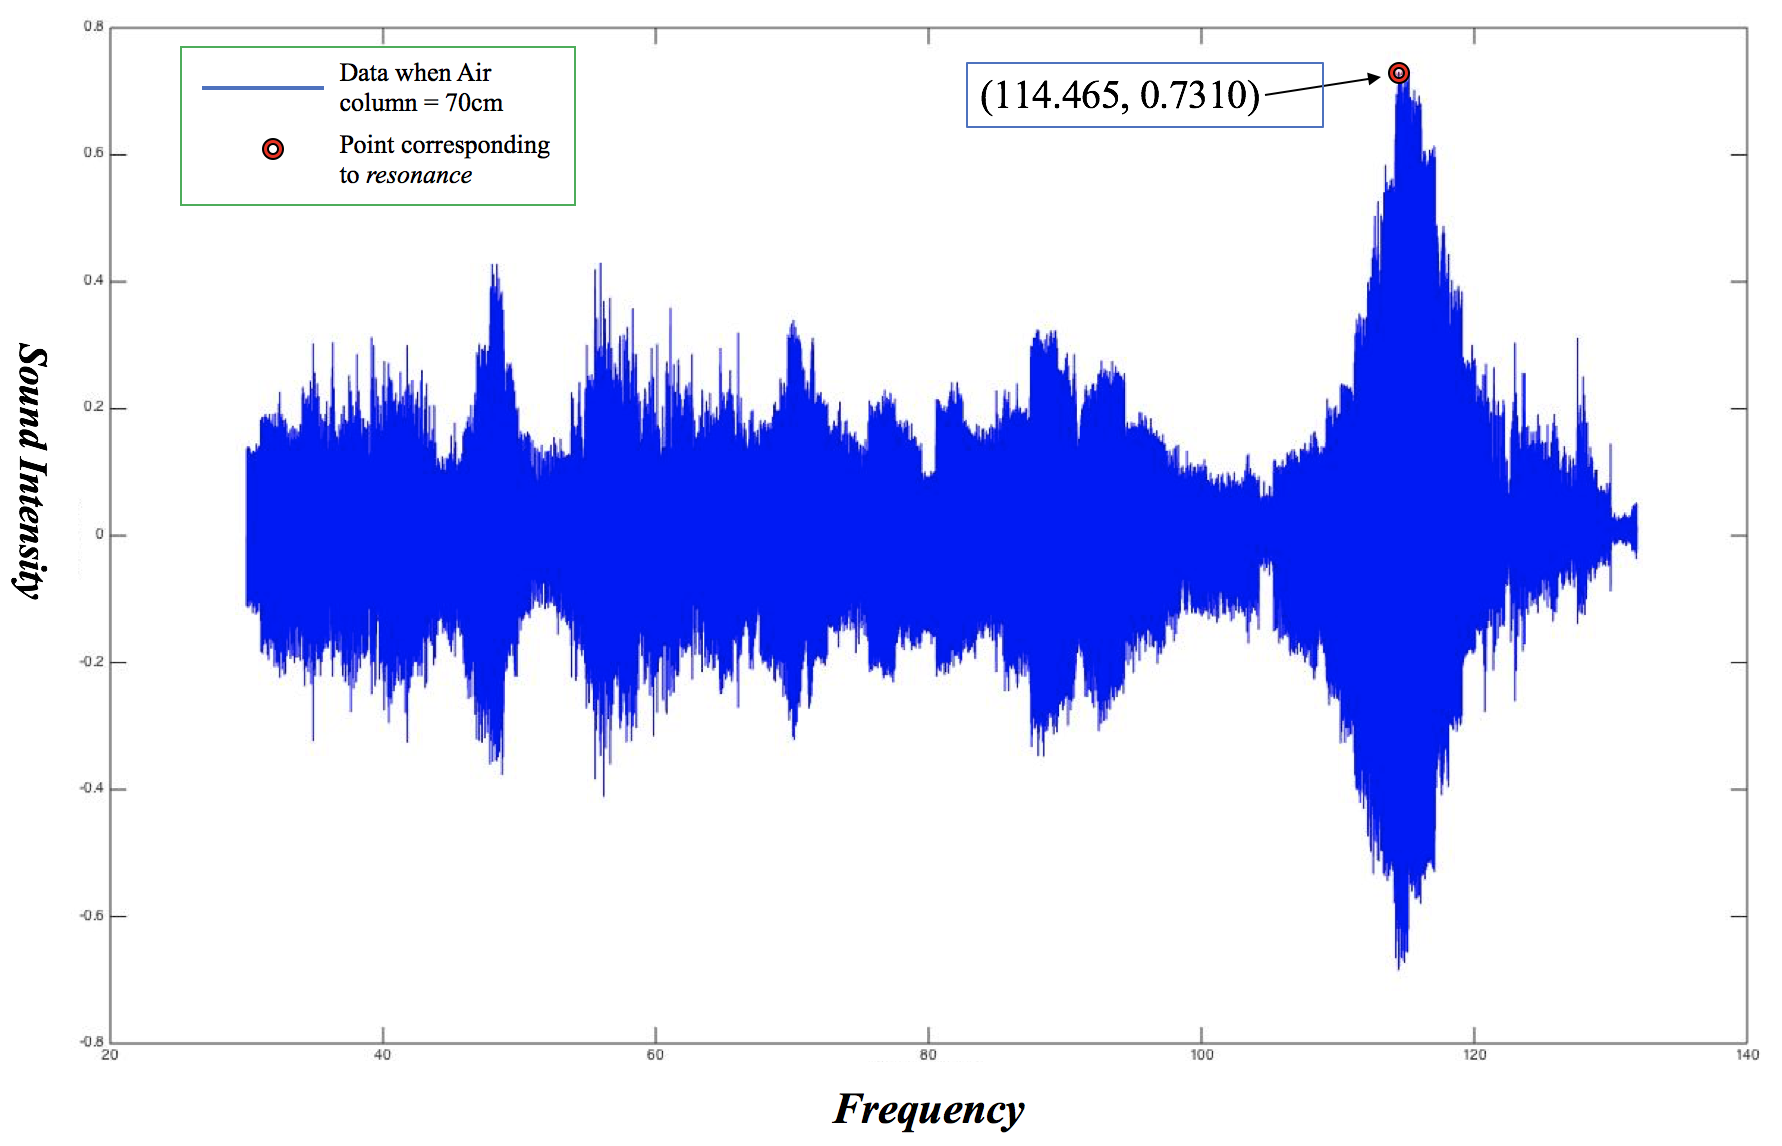
\includegraphics[width=13cm]{Exp_9_graph}
\caption{$Frequency-Intensity$ Graph for $70$cm tube}
\label{$Frequency-Intensity$ Graph for $70$cm tube}
\end{figure}


\section{Data and Error Analysis:}
This section usually should be written no less than 3 pages-long. Derive and explain all the details about data and error analysis here. Always write good math and good English. For details please refer to the reading materials
\begin{quotation}
http://web.stanford.edu/class/ee364b/latex_templates/template_notes.pdf
\end{quotation}

\section{Conclusion}
Briefly conclude and summarize the high-level points. This section should be no longer than half-page.






\end{document}
